% !TEX encoding = UTF-8
% !TEX TS-program = pdflatex
% !TEX root = ../arsclassica.tex
% !TEX spellcheck = it-IT

%************************************************
\chapter{Esperimenti numerici}\label{cap:esperimenti}
%************************************************
\omissis{}
% introdurre concetti del capitolo (dataset, e quindi tsis + sperimentazione)
% introdurre modalità di sperimentazione
% introdurre cross-validation

\section{\Ds{1}}\label{sec:dataset-1}
Lo scopo di questa sezione è presentare il \ds{1} e i risultati di classificazione e apprendimento strutturale ottenuti (si vedano rispettivamente i capitoli~\vref{cap:ctbnc,cap:structurallearning}) utilizzando tale insieme di \emph{\keyword{dati completi}} come input.

\subsection{Modello TSIS}\label{subsec:tsis-simple-model}
Al fine di introdurre il \ds{1} è necessario presentare la rete stradale \acs{TSIS} e il relativo modello di simulazione \acs{CORSIM} da cui esso è stato generato.

\begin{sidewaysfigure}
\centering
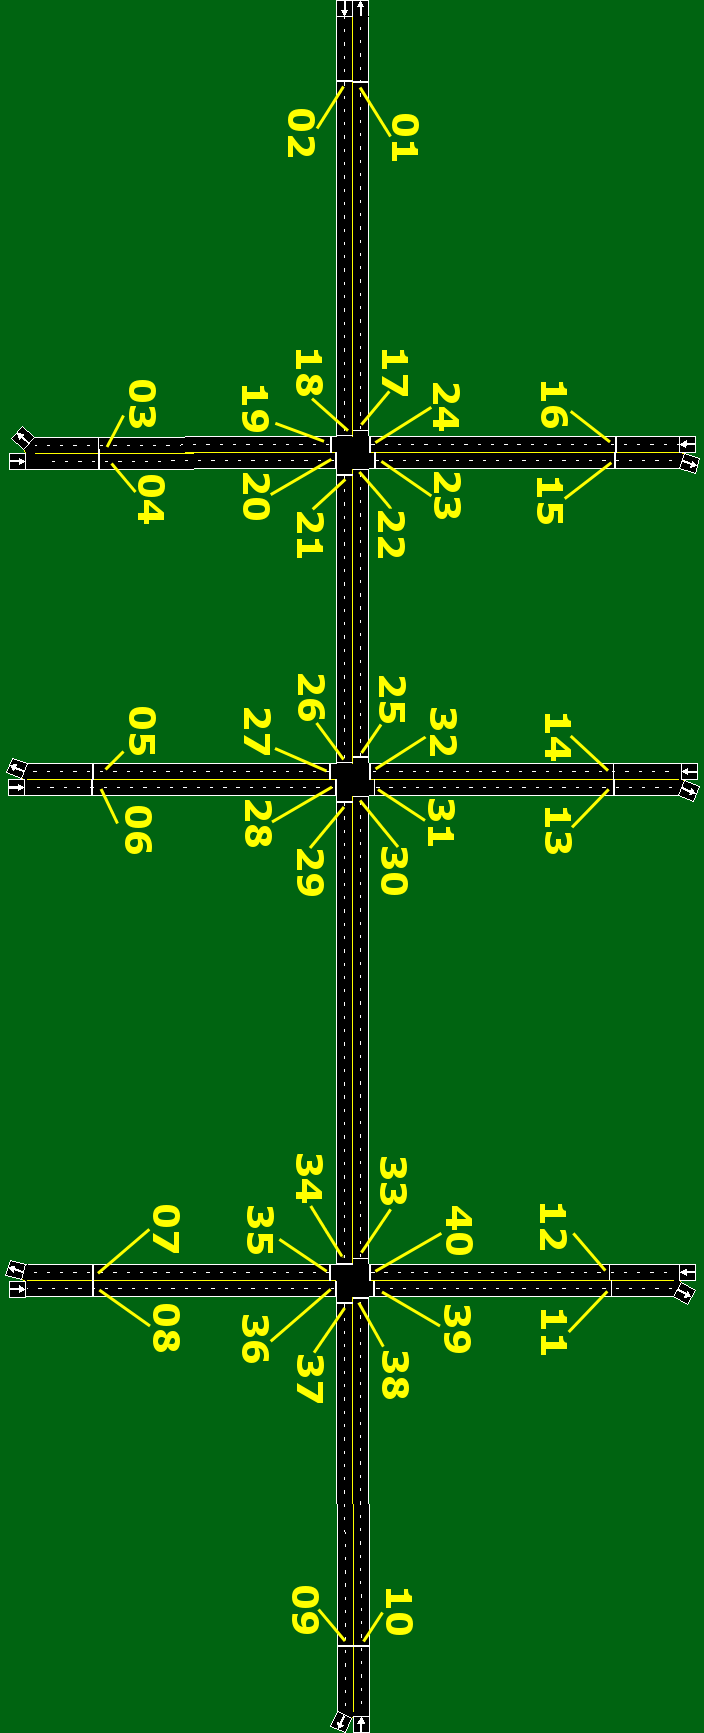
\includegraphics[width=1\columnwidth]{tsis-model-simple}
\caption[Rete stradale del \ds{1}]{File \acs{TNO} rappresentante la rete stradale da cui viene generato il \ds{1}.}
\label{fig:tsis-model-simple}
\end{sidewaysfigure}

%immagine piano semaforico? no
%dire che ci sono (e dove sono) i semafori (l'immagine non li contiene), al massimo incollarli sull'immagine ...
%spiegare come è fatto

\subsection{Risultati}
\omissis{}

%see: https://gist.github.com/leodido/5990626

\section{\Ds{2}}\label{sec:dataset-2}
\omissis{}

\subsection{Modello TSIS}\label{subsec:tsis-monza-model}
\omissis{}

%varianti del dataset utilizzate

\subsection{Risultati}
\omissis{}



%see: https://gist.github.com/leodido/5733991

%risultati:
%apprendimento
%classificazione (cross-validated)
%apprendimento strutturale (cross-validated)